% Définition du répertoire contenant les images
\graphicspath{{IMAGE/}}


% FRAME Intro
\begin{frame}


\includegraphics[width=12cm]{Logos.pdf}

\vfill

\begin{center}

\vspace*{1.5cm}

\LARGE
\textbf{Accessibilité}

\vspace*{2.5cm}

\large

\textbf{Hadrien Commenges}

{\small

\vspace*{0.1cm}

\url{hadrien.commenges@univ-paris1.fr}}

\end{center}

\end{frame}


% FRAME
\begin{frame}{Cas d'application}


\begin{block}{Accessibilité}
L'accessibilité désigne l'accès potentiel: accès d'un agent potentiel à une ressource existante, accès d'un agent existant à une ressource potentielle, accès potentiel à l'espace. 
\end{block}

\textbf{Deux acceptions de l'accessibilité:}

\begin{enumerate}
  \item \textbf{Accès à l'espace:} effort nécessaire pour que des agents accèdent à un lieu. Synonyme de \textbf{desserte}, ce type de mesure dépend du réseau (infrastructure + service) et de la capacité de l'agent à se mouvoir.
  \item \textbf{Accès à la ressource:} effort nécessaire pour que des agents accèdent à une ressource. Ce type de mesure dépend à la fois du réseau, de la capacité de l'agent à se mouvoir et de la \textbf{distribution spatiale de la ressource}.
\end{enumerate}

~

\textbf{Quel type d'information géographique est concerné?}

$\rightarrow$ \textit{TYPE 1, 2, 3, 4, 5}

\end{frame}



% FRAME
\begin{frame}{Distance et interaction}

\begin{itemize}
  \item Le concept clé est la \textbf{friction} (\textit{impedance}), la distance est la mesure de la friction.
  \item L'interaction spatiale être abordée de deux façons: \textbf{relations entre lieux} (flux) ou \textbf{attraction/influence d'un lieu sur les autres lieux}. 
  \item Les modèles d'accessibilité font partie du second type, on peut parler de \textbf{modèles de position}. 
\end{itemize}

\end{frame}



% FRAME
\begin{frame}{Points de vue et contraintes}

\textbf{Deux points de vue pour calculer l'accessibilité:}

\begin{enumerate}
  \item \textbf{Accès unipolaire:} mesure l'accessibilité pour un point d'origine ou de destination.
  \item \textbf{Accès mulitpolaire:} mesure l'accessibilité ``moyenne'' pour l'ensemble des points d'origine et de destination.
\end{enumerate}

~

\textbf{Deux objectifs ou contraintes:}

\begin{enumerate}
  \item \textbf{Temps connu / Stock inconnu:} combien de supermarchés sont accessibles en moins de 10 mn à pied?
  \item \textbf{Temps inconnu / Stock connu:} combien de temps est nécessaire pour disposer d'un bassin d'emploi de 1000 travailleurs?
\end{enumerate}

\end{frame}


% FRAME
\begin{frame}{Types de sorties}

\textbf{Trois types (au moins) de sorties numériques et cartographiques:}

\begin{figure}
  \includegraphics[width=12cm]{TroisSorties.pdf}
\end{figure}


\end{frame}



% FRAME
\begin{frame}{Types d'approches}

\begin{figure}
  \includegraphics[width=8.5cm]{QuatreAcces.pdf}
\end{figure}

$\rightarrow$ L'accessibilité est presque toujours \textbf{calculée sur le réseau}, il faut donc faire un détour par l'\textbf{analyse de graphe} (voir cours correspondant).


\end{frame}



% FRAME
\begin{frame}{Types d'information d'information d'entrée}

\begin{figure}
  \includegraphics[width=12cm]{Semis.pdf}
\end{figure}

\end{frame}


% FRAME
\begin{frame}{Types d'information d'information d'entrée}

\begin{figure}
  \includegraphics[width=12cm]{SemisExpliq.pdf}
\end{figure}

\end{frame}


% FRAME
\begin{frame}{Types d'information d'information d'entrée}

Les notions d'agent et de ressource sont génériques: \textbf{tout peut être agent, tout peut être ressource}.

~

\begin{figure}
  \includegraphics[width=10cm]{AgentRessource.pdf}
\end{figure}

\end{frame}


% FRAME
\begin{frame}{Binaire vs. gravitaire}

\textbf{Accessibilité binaire (présent/absent) et gradient d'accessibilité:}

~

\begin{figure}
  \includegraphics[width=12cm]{BinaireGravitaire.pdf}
\end{figure}

\end{frame}


% FRAME
\begin{frame}{Paramétrage de la friction}

\textbf{Choisir une fonction et des paramètres de friction:}

~

\begin{figure}
  \includegraphics[width=12cm]{FrictionDistance.pdf}
\end{figure}

\end{frame}


% FRAME
\begin{frame}{Paramétrage de la friction}

~

\textbf{Un exemple de paramétrage} sur les gammes d'équipements de la BPE:

\begin{figure}
  \includegraphics[width=12cm]{ProbaFreq.pdf}
\end{figure}

\end{frame}


